\documentclass[letterpaper,10pt]{article}

\usepackage{graphicx}                                        
\usepackage{amssymb}                                         
\usepackage{amsmath}                                         
\usepackage{amsthm}                                          

\usepackage{alltt}                                           
\usepackage{float}
\usepackage{color}
\usepackage{url}

\usepackage{balance}
\usepackage[TABBOTCAP, tight]{subfigure}
\usepackage{enumitem}
\usepackage{pstricks, pst-node}

\usepackage{geometry}
\geometry{textheight=8.5in, textwidth=6in}

\usepackage{tikz}
\usetikzlibrary{arrows,automata}

%----------------------------------------------------------------------------------------
%       Box arround answers use: 
%		\begin{mdframed}[style=MyFrame]
%		\end{mdframed}
%----------------------------------------------------------------------------------------
\usepackage{etex}
\usepackage{tikz}
\usepackage{tikz-qtree}

\usepackage[framemethod=TikZ]{mdframed}
\mdfdefinestyle{MyFrame}{%
    innertopmargin=\baselineskip,
    innerbottommargin=\baselineskip,
    innerrightmargin=20pt,
    innerleftmargin=20pt,
    backgroundcolor=gray!5!white,
    splitbottomskip = 5mm,
    splittopskip = 5mm,
    skipabove=5mm}
    
%----------------------------------------------------------------------------------------
%         Setting for importing code files
%     http://en.wikibooks.org/wiki/LaTeX/Source_Code_Listings
%----------------------------------------------------------------------------------------

\usepackage{import}
\usepackage{listings}
\usepackage{color}

\definecolor{mygreen}{rgb}{0,0.6,0}
\definecolor{mygray}{rgb}{0.5,0.5,0.5}
\definecolor{mymauve}{rgb}{0.58,0,0.82}

\lstset{ %
  backgroundcolor=\color{white},   % choose the background color; you must add \usepackage{color} or \usepackage{xcolor}
  basicstyle=\small,        % the size of the fonts that are used for the code
  breakatwhitespace=false,         % sets if automatic breaks should only happen at whitespace
  breaklines=true,                 % sets automatic line breaking
  captionpos=b,                    % sets the caption-position to bottom
  commentstyle=\color{mygreen},    % comment style
  deletekeywords={...},            % if you want to delete keywords from the given language
  escapeinside={\%*}{*)},          % if you want to add LaTeX within your code
  extendedchars=true,              % lets you use non-ASCII characters; for 8-bits encodings only, does not work with UTF-8
%  frame=single,                    % adds a frame around the code
  keepspaces=true,                 % keeps spaces in text, useful for keeping indentation of code (possibly needs columns=flexible)
  keywordstyle=\color{blue},       % keyword style
  language=Octave,                 % the language of the code
  morekeywords={*,...},            % if you want to add more keywords to the set
  numbers=left,                    % where to put the line-numbers; possible values are (none, left, right)
  numbersep=8pt,                   % how far the line-numbers are from the code
  numberstyle=\tiny\color{mygray}, % the style that is used for the line-numbers
  rulecolor=\color{black},         % if not set, the frame-color may be changed on line-breaks within not-black text (e.g. comments (green here))
  showspaces=false,                % show spaces everywhere adding particular underscores; it overrides 'showstringspaces'
  showstringspaces=false,          % underline spaces within strings only
  showtabs=false,                  % show tabs within strings adding particular underscores
  stepnumber=2,                    % the step between two line-numbers. If it's 1, each line will be numbered
  stringstyle=\color{mymauve},     % string literal style
  tabsize=2,                       % sets default tabsize to 2 spaces
  title=\lstname                   % show the filename of files included with \lstinputlisting; also try caption instead of title
}

%----------------------------------------------------------------------------------------

\newcommand{\toc}{\tableofcontents}

\usepackage{hyperref}

\def\name{Drake Bridgewater }
\def\title{Milestone 2: Scanner Design}
\def\subject{CS }
\def\courseNumber{352 }
\def\courseName{TRANSLATORS }
\def\courseInfo{Winter 2015 }%Class Time: MWF X-X:XX AM}
\def\supervisor{Dr. Jennifer \textsc{Parham-Mocello }} % Supervisor's Name

%% The following metadata will show up in the PDF properties
 \hypersetup{
   colorlinks = false,
   urlcolor = black,
   pdfauthor = {\name},
   pdfkeywords = {\title, \subject, \courseNumber, \courseName, \supervisor},
   pdftitle = {\title},
   pdfsubject = {\subject},
   pdfpagemode = UseNone
 }

\parindent = 0.0 in
\parskip = 0.1 in

\begin{document}


\begin{titlepage}

\newcommand{\HRule}{\rule{\linewidth}{0.5mm}} % Defines a new command for the horizontal lines, change thickness here

\center % Center everything on the page
 
%----------------------------------------------------------------------------------------
%        HEADING SECTIONS
%----------------------------------------------------------------------------------------

\textsc{\LARGE Oregon State University}\\[1.5cm] % Name of your university/college
\textsc{\Large \subject \courseNumber - \courseName}\\[0.5cm] % Major heading such as course name
\textsc{\large \courseInfo}\\[1.5cm] % Minor heading such as course title

%----------------------------------------------------------------------------------------
%        TITLE SECTION
%----------------------------------------------------------------------------------------

\HRule \\[0.4cm]
{ \huge \bfseries \title }\\[0.4cm] % Title of your document
\HRule \\[7.5cm]
 
%----------------------------------------------------------------------------------------
%        AUTHOR SECTION
%----------------------------------------------------------------------------------------

\begin{minipage}{0.4\textwidth}
\begin{flushleft} \large
\emph{Author:}\\
\name
\end{flushleft}
\end{minipage}
~
\begin{minipage}{0.4\textwidth}
\begin{flushright} \large
\emph{Professor:} \\
\supervisor
\end{flushright}
\end{minipage}\\[4cm]

% If you don't want a supervisor, uncomment the two lines below and remove the section above
%\Large \emph{Author:}\\
%John \textsc{Smith}\\[3cm] % Your name

%----------------------------------------------------------------------------------------
%        DATE SECTION
%----------------------------------------------------------------------------------------

DUE 01/16/15 (11:59pm)\\
{\large \today}\\[3cm] % Date, change the \today to a set date if you want to be precise

%----------------------------------------------------------------------------------------
%        LOGO SECTION
%----------------------------------------------------------------------------------------

%\includegraphics{Logo}\\[1cm] % Include a department/university logo - this will require the graphicx package
 
%----------------------------------------------------------------------------------------

\vfill % Fill the rest of the page with whitespace

\end{titlepage}

\tableofcontents
\vfill % Fill the rest of the page with whitespace
\newpage


\section{Assignment 1} \hrule
Read the Naive Semantics document and determine what the various types of tokens are required. Now develop a data structure for these tokens.
\begin{mdframed}[style=MyFrame]
The portion of this had me thinking for multiple days and since I am implementing this in python I decided to use a dictionary as it is stored as a hash table accessing the elements and finding the elements will be straight forward. When it came to storing the variables in the correct place I started thinking about scope and actually implemented a way of managing scopes. I have it made so that I can access any new elements get added to the main scope and when a new scope is defined it is added to the dictionary as a dictionary in a dictionary. 
\end{mdframed}


\section{Assignment 2: Finite State Automata} \hrule
The finite state automata (sing. automaton) paradigm is the basis for the design of the scanner. The finite state automata paradigm as describe in theory texts has two registers (or memory locations) that hold the current character and current state. The program for the machine can be displayed in several standard ways; I want to emphasize a graphical presentation because it is easier to change during design.

To understand the programs, we must first understand the machine execution cycle. This is actually not much different from the cycle used in a standard computer.

\begin{mdframed}[style=MyFrame]
Parsing a number: I have decided to include one of my FSAs as it depicts my thinking as to how numbers are parsed \\
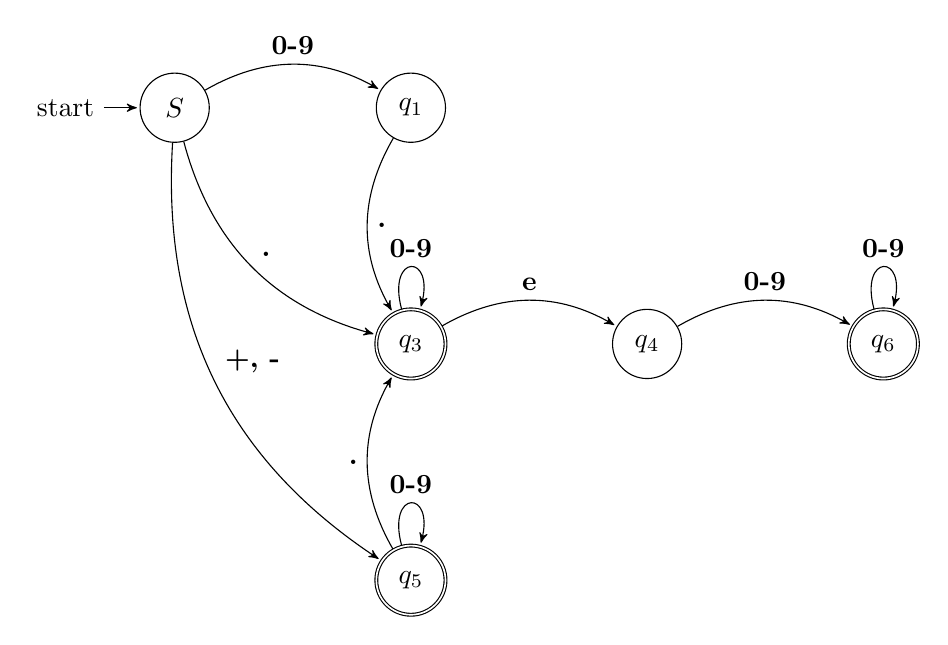
\begin{tikzpicture}[>=stealth',shorten >=1pt,auto,node distance=3cm]
  \node[initial,state] (S)      {$S$};
  \node[state]         (q1) [right of=S]  {$q_1$};
  \node[state, accepting]         
  					   (q3) [below of=q1] {$q_3$};
  \node[state]         
  					   (q4) [right of=q3] {$q_4$};
  \node[state, accepting]         
  					   (q6) [right of=q4] {$q_6$};
  \node[state, accepting]         
  					   (q5) [below of=q3] {$q_5$};


  \path[->] 
  		(S)  edge [bend left]  		node {\textbf{0-9}} 	(q1)
             edge [bend right] 		node {\textbf{.}} 		(q3)
             edge [bend right] 		node {\textbf{+, -}} 	(q5)
        (q1) edge [bend right] 		node {\textbf{.}} 		(q3)
        (q3) edge [loop above] 		node {\textbf{0-9}}		(q3)
             edge [bend left]  		node {\textbf{e}} 		(q4)
        (q4) edge [bend left] 		node {\textbf{0-9}}		(q6)
        (q5) edge [loop above] 		node {\textbf{0-9}}		(q5)
             edge [bend left] 		node {\textbf{.}} 		(q3)
        (q6) edge [loop above] 		node {\textbf{0-9}}		(q6);
\end{tikzpicture}
\end{mdframed}
\section{Assignment 3} \hrule
The technical difference between automaton and machine is that an automaton only gives an accept-reject response while a machine does transformations.

Assignment 2 only develop the yes/no portion of the scanner. The scanner must produce a token as output and therefore, we need to think about the saving of characters, possibly converting some (like integers or special characters in strings), etc. We denote this by the weight.

Modify your output of assignment 2 to reflect the processing to save and convert characters to form tokens.
\begin{mdframed}[style=MyFrame]
This portion was rather easy as I was already storing the data I just had to print the data structure and with python this was easy just calling the print on the dictionary. 
\end{mdframed}


\subsection{Report}
%Handwritten Answers to Milestone Questions:
%Specification (what do you think the purpose of this milestone is)
%Processing (how did you go about solving the problem)
%Testing Requirement (how did you test for correctness)
%Retrospective (what did you learn in this milestone)

\begin{mdframed}[style=MyFrame]
This assignment was to create a scanner that reads source code written in IBTL and figure out if the tokens are accepted in the language. To solve this problem I worked to process words and add them to a list, but quickly realized that a list will not be great at storing token and symbols. Therefore, I implemented a dictionary that would allow finding of symbols quicker; the keys are the different types of and one of the keys contains the scope which contains additional scopes. To make sure that my implementation worked I looked at the FSA and used sequences of tokens that should be accepted and sequences of tokens that should fail. In the end I learned that scanning for tokens character by character is much easier then when you scan by spaces which I was originally thinking. 
\end{mdframed}



\newpage
\subsection{Source For scanner.py}
\lstinputlisting[language=Python]{scanner.py}



\end{document}